\subsection{X-ray fluorescence analyser}
Life on Europa requires an environment that can sustain it. To determine if the water under the ice of Europa can sustain life a chemical analyses of the water is needed. One such analyses is determining what elements are present in the water. For this purpose an X-ray fluorescence analyser is proposed.

\paragraph{Primary objective:}
To detect and quantify what elements are present in the water beneath the ice on Europa.


\subsection{XRF theory}

The X Ray Fluorescence (XRF) analyser irradiates a sample with x rays, and from the samples resulting fluorescence determines what elements are in the sample. 
When an atom is hit by a photon an electron can be knocked out of it’s orbit (primarily  the k shell), the following ‘replacement’ of this electron with an electron from a higher shell  will emit a photon which energy is characteristic for that element, this is called the characteristic x-rays or fluorescent x-rays. To knock an electron out of it’s orbit the incident photon have to be of a higher energy than the binding energy of the electron. The binding energy of electron in the k-shell increases with atomic number Z. 

\begin{figure}[h]
	\centering
	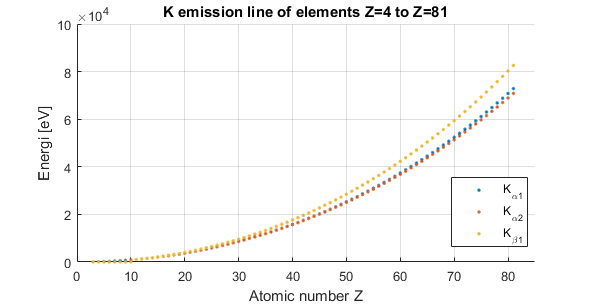
\includegraphics[width=\textwidth]{figures/XRF/Kalpha12Lines.png}
	\caption{$K_{\alpha 1}$, $K_{\alpha 2}$ and $K_{\beta 1}$ emission lines.}
	\label{fig:KalphaEmiLines}
\end{figure}

By measuring the energy of a sample's fluorescence photons, and the intensity at which they occur, the samples constituents and their quantity can be determined. Using this method elements as light as Beryllium (atomic number Z= 4) can be detected. The energy of the characteristic x-rays increase with atomic number, with very low energy x-rays for the light elements, 108eV for Beryllium (Z=4), to very high energies for heavier elements, 22keV for Ag (Z=47) and 71keV for Hg (Z=80).
The key components in an XRF analyser is the x-ray source and the x-ray detector. To increase performance x-ray optics can be added.

\subsubsection{X-ray source}
X-rays can be generated by bombarding a metal object with electron which have been accelerated through an electric field of up to several thousands volts. This is done in a vacuum tube called an x-ray tube, where a high voltage (100-80000V) is applied over a cathode and an anode. The electron are emitted from the cathode and when hitting the anode x-rays are emitted. If the electrons hit the anode with an energy higher than the anode atoms binding energy, they can knock inner electrons out of the orbit of the anodes atoms. The electrons which are knocked out from their orbit form the characteristic x-rays, this results in 'spikes' of high x-ray intensity around the anode metals characteristic x-rays line.
The electrons that do not interact directly with the atoms are slowed down in the anode metal and their energy is emitted as bremsstrahlung or braking radiation. The braking radiation form a continuous spectrum, with lower intensity for higher energies.
The intensity of an x-ray source is governed by the voltage applied and the intensity of te electron beam. The shape and direction of the beam is determined by the geometry of the anode, and the size of the electron beam spot on the anode.


\subsubsection{X-ray detector}
Measuring the fluorescent x-rays emitted can be done using two methods: Energy dispersive and wavelength dispersive. 
With the energy dispersive method the x-rays are directed towards a detector, where the x-ray photons induce a current proportional with. This process is repeated for every photon hitting the detector, creating a continuous stream of current pulses. These current pulses are recorded and sorted into discrete energy ranges by a Multi Channel Analyser (MCA). The result is a energy spectrum of the recorded x-ray photons. This method is suiteble for analysers who are designed to detect a range of elements, as it can detect a wide range of energies.
The wavelength dispersive method directs the fluorescent photons to a monochromator or diffractor before they are directed to a detector. The monochromator/diffractor ensures that only a narrow range (in terms of wavelength) of photons reach the detector. The detector used is commonly a photomultiplier which counts the incident photons. the result of an wavelength dispersive analysis is a measurement of the x-ray intensity at a specific wavelength. While multiple measurements can be done covering different wavelength, an energy dispersive method is better suited for this task.
For this mission the energy dispersive method is used.

\subsubsection{Mission specific criteria:}
Doing x-ray spectroscopy on Europa provides unique challenges that needs to be considere, when designing an instrument. The most prominent is:\\
\begin{itemize}
\item Operating at 130bar pressure.
\item Operating in a wet environment.
\item Analysing aqueous solutions.
\end{itemize}
These challenges will be discussed in the following sections.

\paragraph{High pressure environment}
Common XRF analysers consists of vacuum tube instruments, namely an  x-ray tube as X ray source, and the X ray detector. The interface between these instruments vacuum environment and the surrounding environment commonly consists of a thin (~0.1mm) Beryllium window. Beryllium is used because of it low X ray attenuation compared to its strength. When operating under the ice of Europa a vastly stronger window is needed, to be able to withstand the pressure.
Estimating the thickness of a clampedpressure window can be done with the following \citep{High_pressure_window}: 

\begin{equation}
\frac{F_a}{SF} = \frac{K \cdot D^2 \cdot P}{4 \cdot T^2} 
\end{equation}
\begin{equation}
\label{eq:PressureWinT}
T = D \cdot \sqrt{SF \cdot \frac{K}{4}} \cdot \sqrt{\frac{P}{F_a}}
\end{equation}

\noindent$F_a$ is the apparent elastic limit of the material [Pa].\\
SF: safety factor.\\
T: the thickness of the window [m].\\
K: empirical constant (1.125 for clamped windows with flexible fixture).\\
D: unsupported diameter of window [m].\\
P: pressure difference across window [Pa].\\

Using \ref{eq:PressureWinT} a 3mmØ beryllium window ($F_a$ at 240MPa \citep{BeMechanical}) with a safety factor of 8 results in a 1.05mm thick window. The Beryllium window will attenuate the fluorescent x-rays, and lower the detection limits.
Instead of a beryllium plate as a window, a polycapillary x-ray lens can be used. the polycapillary lens would function as the barrier between the vacuum environment and the high pressure environment, and focus/collimate the x-ray beam simultaneously. The polycapillary lens would need testing to make sure it can withstand the pressure. To seal off the end of the capillary tubes a beryllium film of 1-20um thickness could be used (assuming capillary diameter of 3-25um \citep{PolyCapOptics}, SF of 8 and $F_a$ at 240MPa).


\paragraph{Poly capillary optics}
Polycapillary lenses are a collection of thin tubes (capillaries), usually made from borosilicate glass, which direct x-rays through total external reflection. Total external reflection occurs when an incident photon enters the capillary and hits the glass wall at less than the critical angle. this is due to the differences in the refractive index of glass and the gas/vacuum of the capillary. This way any photon entering the tube at less than the critical angle is propagated through the capillary and its trajectory altered depending on the capillary curvature. Polycapillary lenses can be used for focusing or collimating purposes, by adjusting the curvature of the capillaries.
The focusing distance of a polycapillary lens is dependent on the photon energy and the focal spot size. It can be estimated using\citep{PolyCapOptics}:

\begin{equation}
FD = S \cdot \frac{E}{60}
\end{equation}

\noindent FD: focal distance [m].\\
S: spot size [m].\\
E: photon energy [eV].\\

The smallest focal spot commonly used is around 10um.
If used for focusing different energies the focusing distance will change. If used for focusing the fluorescent x-rays of a sample in the XRF analyser, a poly capillary lens will result in a focal ‘column’ of focal spots for the different energies. 


\paragraph{Wet environment}
As the environment is expected to be wet, it is necessary to consider the potential loss in the water. The sample is expected to be an aqueous solution, and there will be an attenuation of the X rays moving from the center of the sample outwards. 

The sample being an aqueous solution thus limits what we can detect further from the surface of the sample. The fluorescent X rays of the lighter elements (lower Z)  are lower in energy and will be attenuated more, as seen in \ref{fig:AttnH2O}.

\begin{figure}[h]
	\centering
	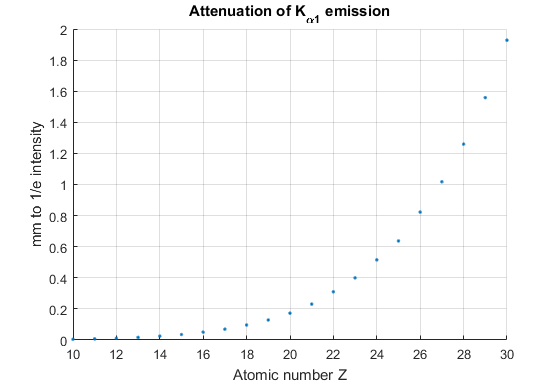
\includegraphics[width=0.8\textwidth]{figures/XRF/AttnOfKaplha.png}
	\caption{Attenuation of x-rays in H2O, in distance to 1/e intensity, for different elements\citep{XRay_Attn_H2O}}
	\label{fig:AttnH2O}
\end{figure}

% [INCLUDE PLOT OF WATER ATTENUATION OF X RAYS, AND WHERE THE ELEMENTS LIE IN THIS PLOT]  [Source http://henke.lbl.gov/optical_constants/ for attn & http://www.med.harvard.edu/jpnm/physics/refs/xrayemis.html for Kalpha line]

Detecting elements in the lower region, lighter than Cobalt (Z=27, $K_{\alpha 1}$ at 6.9keV), could prove difficult through more than 1 mm of water, due to the fluorescent photons being attenuated very heavily. 


\paragraph{Compton scattering in water}
When subjecting an aqueous sample to X ray irradiation, Compton scattering have to be taken into account. The Compton scattering results in reflected X ray photons depending on the incident photons energy, and the reflected angle. Energy of the scattered photons can be estimated with \ref{eq:ComtonEQ} \citep{ComptonScatt}:

\begin{equation}
\label{eq:ComtonEQ}
hv' =  \frac{hv}{ 1+alpha*(1-cos(theta)) }
\end{equation}

\noindent hv': energy of the reflected photon.\\
hv: energy of the incident photon.\\
alpha: $\frac{hv}{electron rest energy (0.511MeV)}$ \\
 
The scattered photons are scattered evenly in all directions. Thus the scattering results in a distorted mirror of the incident photon energy spectrum. If the incident spectrum is concentrated in a narrow energy band, it can mask some fluorescent x-rays in the sample.

%If an x-ray source of 17.5 keV is used, the resulting compton peak will be in the range of 16.3keV to 17.5keV. This will intersect with the Kalpha line of Yttrium (Z: 39) and Zirconium (Z: 40), and possible further depending the consistency, in terms of photon energy, of the x-ray source. It is thus important to pick an x-ray source that will not obscure important elements with the compton scattered radiation.



